\chapter[X-box (Uthus)]{X-box}
\label{sec:xbox}

\begin{figure}[h]
  \centering \fbox{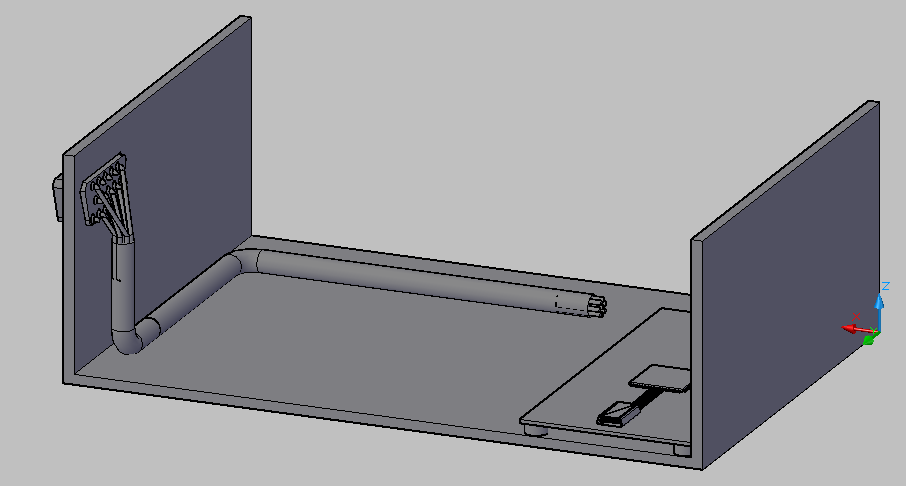
\includegraphics[width=0.8\linewidth]{fig/x-boxsalangt.png}}
  \caption[Skisse av <<X-box>>]{Skisse av <<X-box>>, laget i AutoCAD}
  \label{fig:xboxACad}
\end{figure}

\begin{quote}\it
  \textbf{Sammendrag:} Inneholder en kort beskrivelse av hvordan <<X-box>>-en
  ble laget og hva den brukes til. Bakgrunnen til at <<X-box>>-en ble laget er
  gitt i kapittel~\ref{sec:hodeboyle}. <<X-box>>-en skal inneholde elektronikken
  som behandler dataen fra hodeb�ylen, og sender den videre til PC-en.
\end{quote}

\section{Problemstilling}

Det var et behov for et mellomledd mellom selve musen (hodeb�ylen,
kap.~\ref{sec:hodeboyle}) og datamaskinen. Dette bindingspunktet m�tte enkelt
kunne kobles til hodeb�ylen via COM-port og samtidig kunne kobles videre via USB
til PC-en. Det m�tte inneholde kretskortet til mikroprosessoren.

\section{Gjennomf�ring}

Prosjektgruppen fant ut at det skulle lages en boks som skulle ha to kontakter:
En COM-port som skulle kobles til hodeb�ylen, den andre kontakten skulle v�re
USB for � kommunisere videre inn til datamaskinen. Inne i boksen skulle det ogs�
v�re plass til kretskortet, samt til � sette p� testutstyr for � resette/justere
koden underveis. Det ble brukt en metalplate som b�ydes 90\degree\ p� hver side.
Dette utgjorde underlaget til boksen og 2 <<vegger>>. Kretskortet ble festet
inne i boksen ved hjelp av gaffateip, og plasseringen av kortet var s� n�r den
ene kanten uten <<vegg>> slik at den lett kan kobles til USB-kabelen (som en kan
se p� fig.~\ref{fig:xboxtopp}). Siden det skulle v�re COM-kontakt mot
hodeb�ylen, ble det laget et hull i den ene siden hvor COM-porten ble satt inn.
Det ble strukket ledninger som p� den ene siden var loddet fast til kretskortet,
den andre enden til COM-porten. N� var det alts� bare � koble i headsettet p�
den ene siden, og maskinen med USB p� den andre. <<That's Plug `n' Play!>>

\begin{figure}[h]
  \centering
  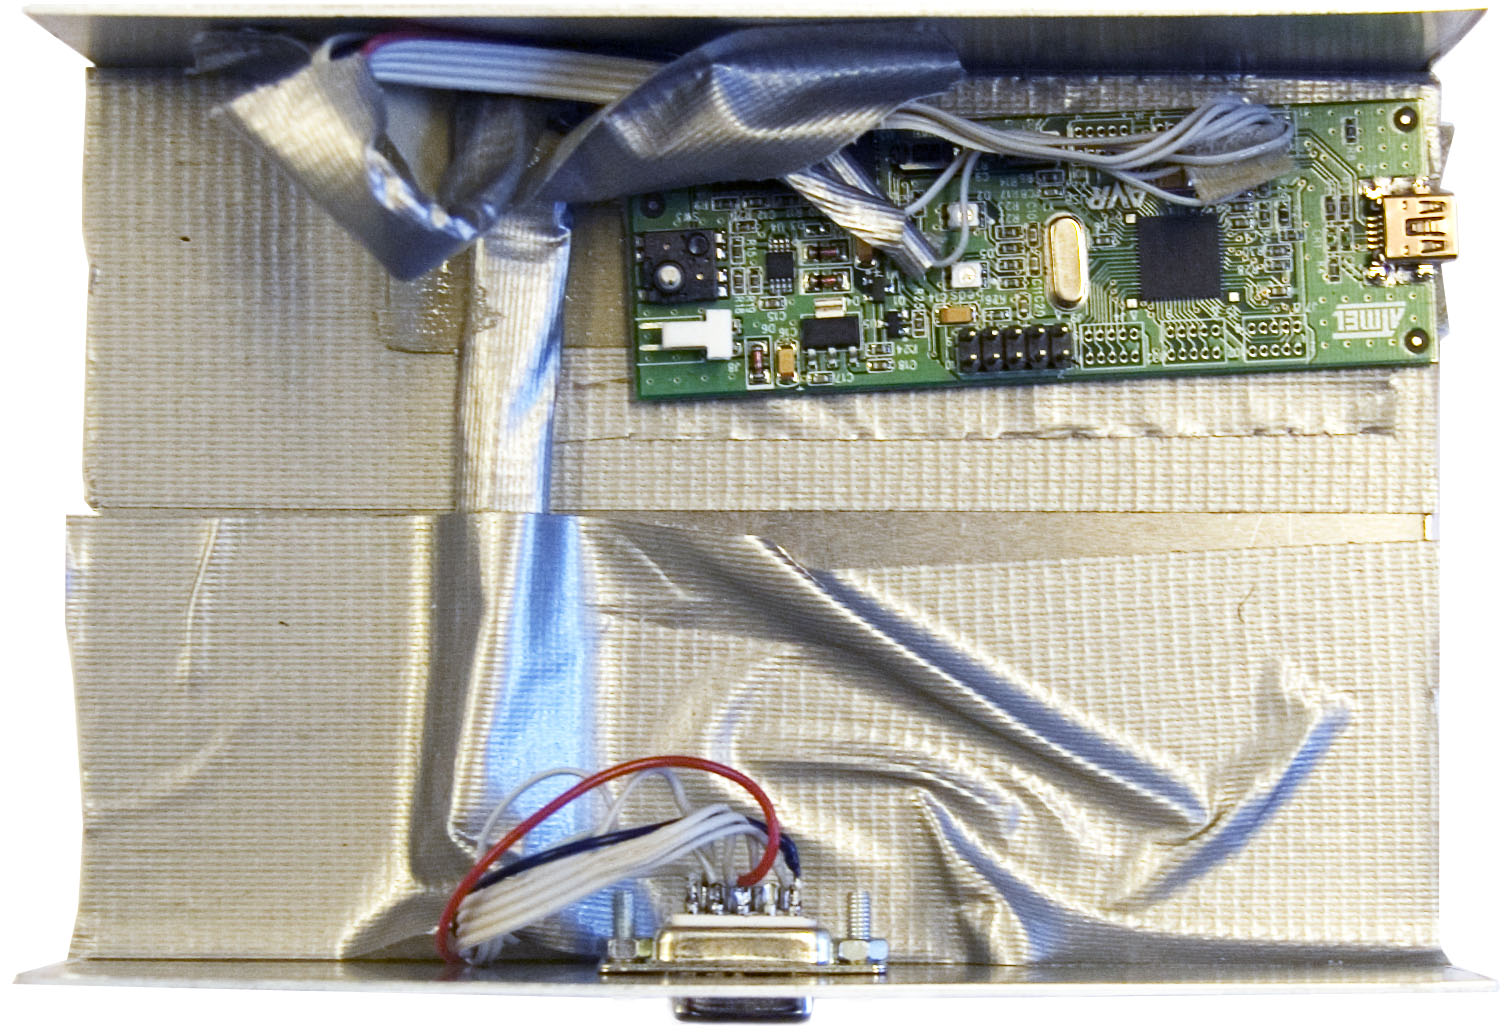
\includegraphics[width=0.6\linewidth]{fig/x-box2.jpg}
  \caption{Bilde av <<X-box>> fra toppen}
  \label{fig:xboxtopp}
\end{figure}

\section{Resultat}

En boks som skal v�re et bindeledd mellom PC-en og musen
(figur~\ref{fig:xboxferdig}. Den har en COM-port som var gruppens l�sning for �
p� en enkel m�te koble til hodeb�ylen. Videre g�r data fra hodeb�ylen inn til
kretskortet, og videre til maskinen som utf�rer �nskede operasjoner.

\begin{figure}[h]
  \centering
  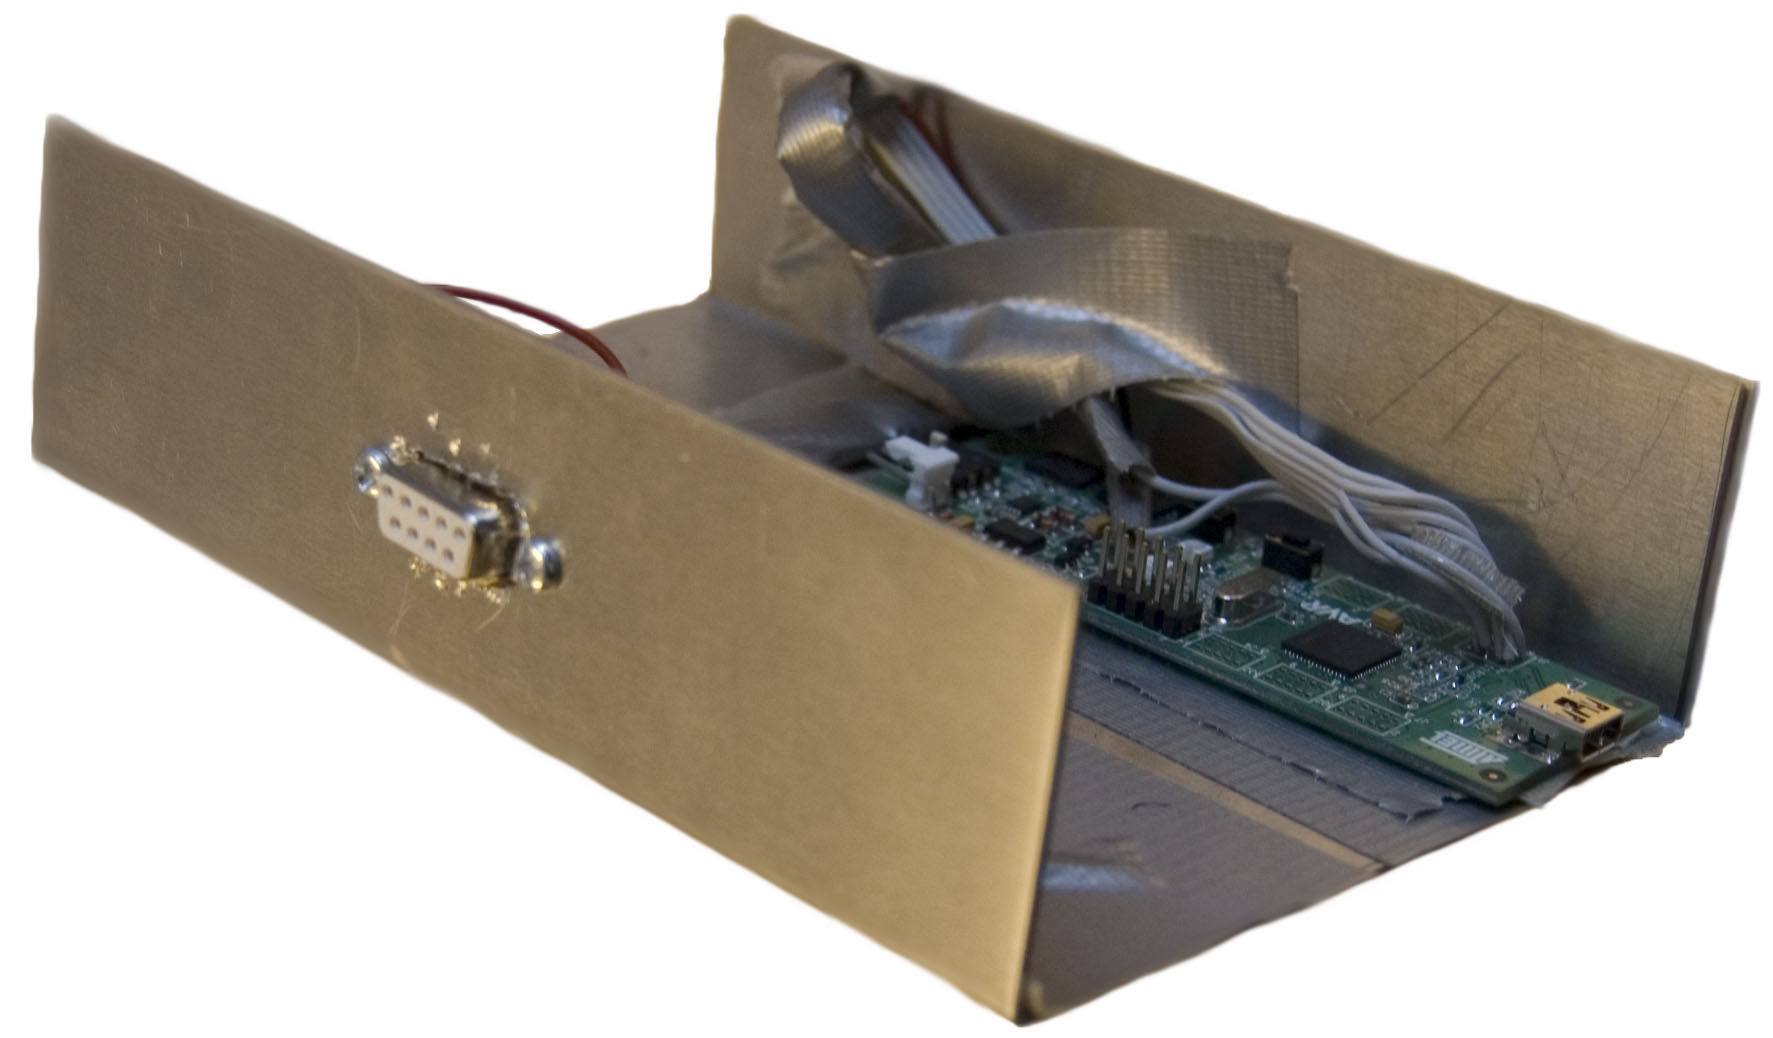
\includegraphics[width=0.6\linewidth]{fig/x-box1.jpg}
  \caption{Bilde av ferdig <<X-box>>}
  \label{fig:xboxferdig}
\end{figure}
